% !TEX program = xelatex
%% Requires compilation with XeLaTeX or LuaLaTeX
\documentclass[10pt,xcolor={table,dvipsnames},t]{beamer}
\usepackage{biblatex}
\usepackage{caption}
\setbeamertemplate{caption}[numbered]
\addbibresource{reference.bib}
\usepackage{hyperref}
\hypersetup{ 
pdfpagemode=FullScreen,  
colorlinks=true,linkcolor=blue}
\usepackage{enumerate}
\usepackage{algorithm}
\usepackage{algpseudocode}
\usepackage{listings}
\usepackage{xcolor}

\definecolor{codegreen}{rgb}{0,0.6,0}
\definecolor{codegray}{rgb}{0.5,0.5,0.5}
\definecolor{codepurple}{rgb}{0.58,0,0.82}
\definecolor{backcolour}{rgb}{0.95,0.95,0.92}

\lstdefinestyle{mystyle}{
    backgroundcolor=\color{backcolour},   
    commentstyle=\color{codegreen},
    keywordstyle=\color{magenta},
    numberstyle=\tiny\color{codegray},
    stringstyle=\color{codepurple},
    basicstyle=\ttfamily\footnotesize,
    breakatwhitespace=false,         
    breaklines=true,                 
    captionpos=b,                    
    keepspaces=true,                 
    numbers=left,                    
    numbersep=5pt,                  
    showspaces=false,                
    showstringspaces=false,
    showtabs=false,                  
    tabsize=2
}

\lstset{style=mystyle}

% Flow chart config
\usepackage{tikz}
\usetikzlibrary{calc,trees,positioning,arrows,fit,shapes,calc,tikzmark,matrix}
\usepackage{eso-pic}
\usetikzlibrary{shapes.geometric, arrows}
\tikzstyle{startstop} = [rectangle, rounded corners, minimum width=3cm, minimum height=1cm,text centered, draw=black, fill=red!30]
\tikzstyle{io} = [trapezium, trapezium left angle=70, trapezium right angle=110, minimum width=3cm, minimum height=1cm, text centered, draw=black, fill=blue!30]
\tikzstyle{process} = [rectangle, minimum width=3cm, minimum height=1cm, text centered, draw=black, fill=orange!30]
\tikzstyle{decision} = [diamond, minimum width=3cm, minimum height=1cm, text centered, draw=black, fill=green!30]
\tikzstyle{arrow} = [thick,->,>=stealth]

\usetheme{UCBerkeley}

\title[Your Short Title]{STMC Coding Team Training}
\subtitle{Lesson 8: Data Structure II}
\author{Tsai Yun Chen}
%\institute{}
\date{\today}

\begin{document}

\begin{frame}
  \titlepage
\end{frame}

% Uncomment these lines for an automatically generated outline.
%\begin{frame}{Outline}
%  \tableofcontents
%\end{frame}

\section{Class Goal}

\begin{frame}{Goal today}
Today we will continue the topic of data structure, in particular we will study the commonly used structure: stack, queue. Then we will look into different applications of these data structure.
\begin{itemize}
  \item A recap on linked-list
  \item A new implementation
  \item Stack and Queue, LIFO and FIFO
  \item implementing stack and queue using linked-list
  \item application: formula parser
  \item Shunting yard algorithm (simplified)
  \item HKOI problem: The Josephus Problem
\end{itemize}
\end{frame}

\begin{frame}{Linked List}
  Recall what we have learnt at the end of last lecture.
  \begin{figure}[h!]
    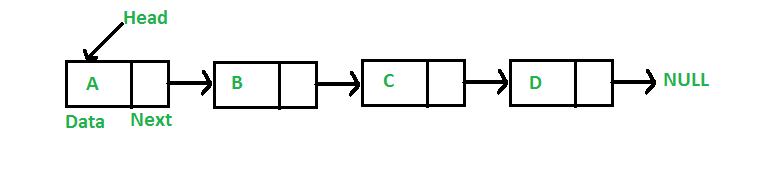
\includegraphics[width=0.7\textwidth]{img/Linkedlist.png}
    \caption{Linked List(\href{https://www.geeksforgeeks.org/data-structures/linked-list/}{Source})}
  \end{figure}
\end{frame}

\begin{frame}[fragile]{Naive Implementation}
  We have a simple implementation last time,
\begin{lstlisting}[language=python]
  class LinkedList:
    def __init__(self):
      self.data=None
      self.next=None
    def insert(self,data):
      if self.data==None:
        self.data=data
        self.next=LinkedList()
      else:
        self.next.insert(data)
\end{lstlisting}
\end{frame}

\begin{frame}{Some problem}
  Some problem with the previous implementation,
  \begin{itemize}
    \item it takes $O(n)$ time to insert one data to the end
    \item which makes no difference with array
    \item we need also remove of data
    \item Let's slightly improve it!
  \end{itemize}
\end{frame}

\begin{frame}[fragile]
\begin{lstlisting}[language=python]
  class llnode:
    def __init__(self):
      self.data=None
      self.prev=None #newly added
      self.next=None
  class ll:
    def __init__(self):
      self.head=llnode() #empty node
      self.tail=self.head
      self.size=0
    def Insert(self,data,mode='front'):
      if mode=='front':
        temp=llnode()
        temp.data=data
        temp.next=self.head
        self.head.prev=temp
        self.head=temp
      elif mode=='end':
        temp=llnode()
        temp.data=data
        self.tail.next=temp
        temp.prev=self.tail
        self.tail=temp
      else:
        raise Exception("Unrecognized mode of insertion")
\end{lstlisting}
\end{frame}

\begin{frame}[fragile]
\begin{lstlisting}[language=python]
  def Pop(self,mode='front'):
    if mode=='front':
      if self.size==0:
        raise Exception("Popping empty list")
      temp=self.head
      self.head=self.head.next
      self.head.prev=None
      return temp.data
    elif mode=='end':
      if self.size==0:
        raise Exception("Popping empty list")
      temp=self.tail
      self.tail=self.head.tail.prev
      self.tail.next=temp.next
      return temp.data
    else:
      raise Exception("Unrecognized mode of insertion")
\end{lstlisting}
\end{frame}

\begin{frame}{Queue and Stack}
  Now we are ready to explore another new data structure. We are going to explore two classic and extremely useful data structures, namely queue and stack, these two data structures are inspired from our daily life experience as we will see later
  \begin{enumerate}
    \item Queue
    \begin{itemize}
      \item Data are stored in the order of adding them
      \item Just like you are queuing at a store, first-come-first-serve
      \item We also called this type of operation First-In-First-Out (FIFO)
      \item Commonly used in task-scheduling and best-solution searching
    \end{itemize}
    \item Stack
    \begin{itemize}
      \item Data are stored in the \textbf{reverse} order of adding them
      \item Just like you are stacking up a bunch of paper on table, the first one will be at the bottom
      \item We also called this type of operation Last-In-First-Out (LIFO) or First-In-Last-Out (FILO)
      \item Commonly used in parsing, recursive process and fast solution searching
    \end{itemize}
  \end{enumerate}
\end{frame}

\begin{frame}{Queue, a illustration}
  \begin{figure}[h!]
    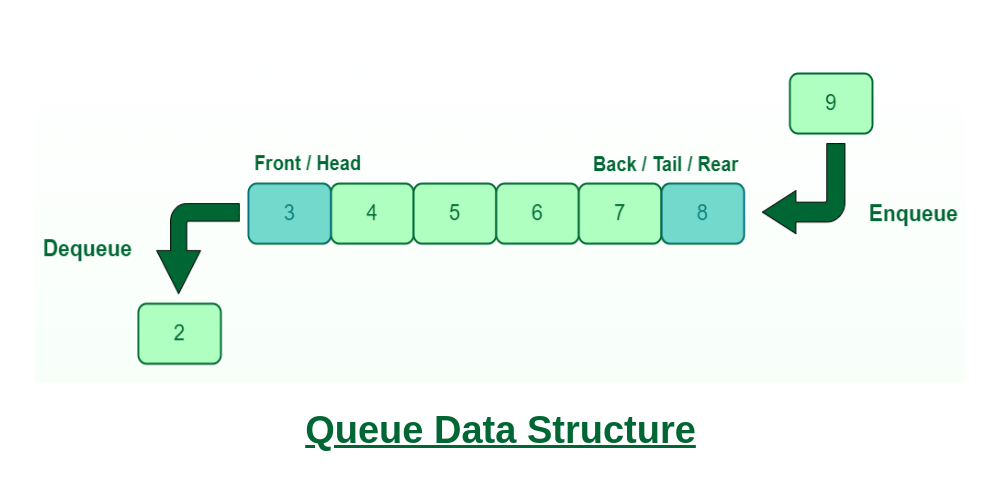
\includegraphics[width=0.7\textwidth]{img/queue.png}
    \caption{Queue(\href{https://www.geeksforgeeks.org/queue-data-structure/}{Source})}
  \end{figure}
\end{frame}

\begin{frame}{Stack, a illustration}
  \begin{figure}[h!]
    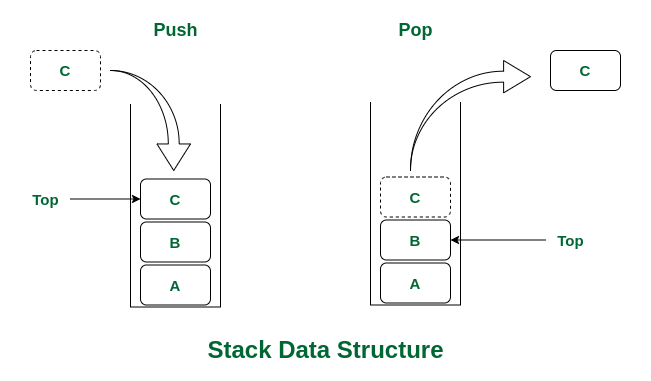
\includegraphics[width=0.7\textwidth]{img/stack.png}
    \caption{Stack(\href{https://www.geeksforgeeks.org/stack-data-structure/}{Source})}
  \end{figure}
\end{frame}

\begin{frame}{Implementation}
  Now let's do the implementation, since the major feature of such strctures are update and query (FIFO,FILO), it makes sense for us to utilize the linked list we just learnt (and that's why we are introducing it). I will do the stack as an example and the queue will be your exercise. What we will need is
  \begin{itemize}
    \item A class holding a structure \texttt{stack}
    \item operator pop(): removes a data from the top and return it
    \item operator push(): add a data to the top
    \item operator top(): return the data currently at top without removing it
    \item operator empty(): return true of the stack is empty now, else return false
    \item operator size(): return the current size of the stack
  \end{itemize}
\end{frame}

\begin{frame}[fragile]
\begin{lstlisting}[language=python]
  class stack:
    def __init__(self):
      self.data=ll()
    def pop(self):
      return self.data.Pop()  #default popping from the front
    def push(self):
      self.data.Insert()  #default insert to the front
    def top(self):
      if self.data.size>0: 
        return self.data.head.data
      else:
        raise Exception('Accessing empty stack')
    def empty():
      return self.data.size==0
    def size():
      return self.data.size
\end{lstlisting}
The implementation is actually pretty simple with the help of linked-list.
\end{frame}

\begin{frame}{Implementation Queue}
  Now it's your turn, let's try to implement a queue, make sure you work it out since we will be using it later.
\end{frame}

\begin{frame}{Application of Stack: Formula Parser}
  Now let's look at some application, consider now we are designing a calculator, our job is to receive a formula, evaluate it and return the answer. For example the input might be 
  $$1+2+3$$
  Then our program should be able to evaluate the answer $6$ and return it.\\
  But the problem is there might be formula like this
  $$1+2\times 3$$
  Then we must perform the $\times$ first and then perform the $+$. In general this problem could be hard to solve and there is a famous algorithm called the Shunting-yard algorithm (Developed by Dijkstra, a great computer scientist).
\end{frame}

\begin{frame}{Shunting-yard algorithm}
  \begin{columns}
    \begin{column}[T]{0.5\textwidth}
      \begin{figure}
        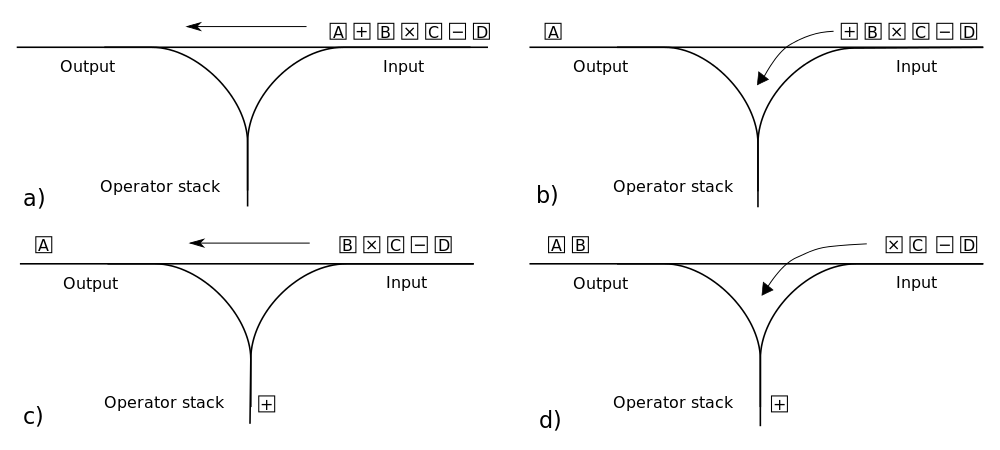
\includegraphics[width=0.7\textwidth]{img/Shunting_yard.png}
        \caption{Shunting-yard algorithm (\href{https://en.wikipedia.org/wiki/Shunting_yard_algorithm}{Source})}
      \end{figure}
    \end{column}
    \begin{column}[T]{0.5\textwidth}
      \begin{figure}
        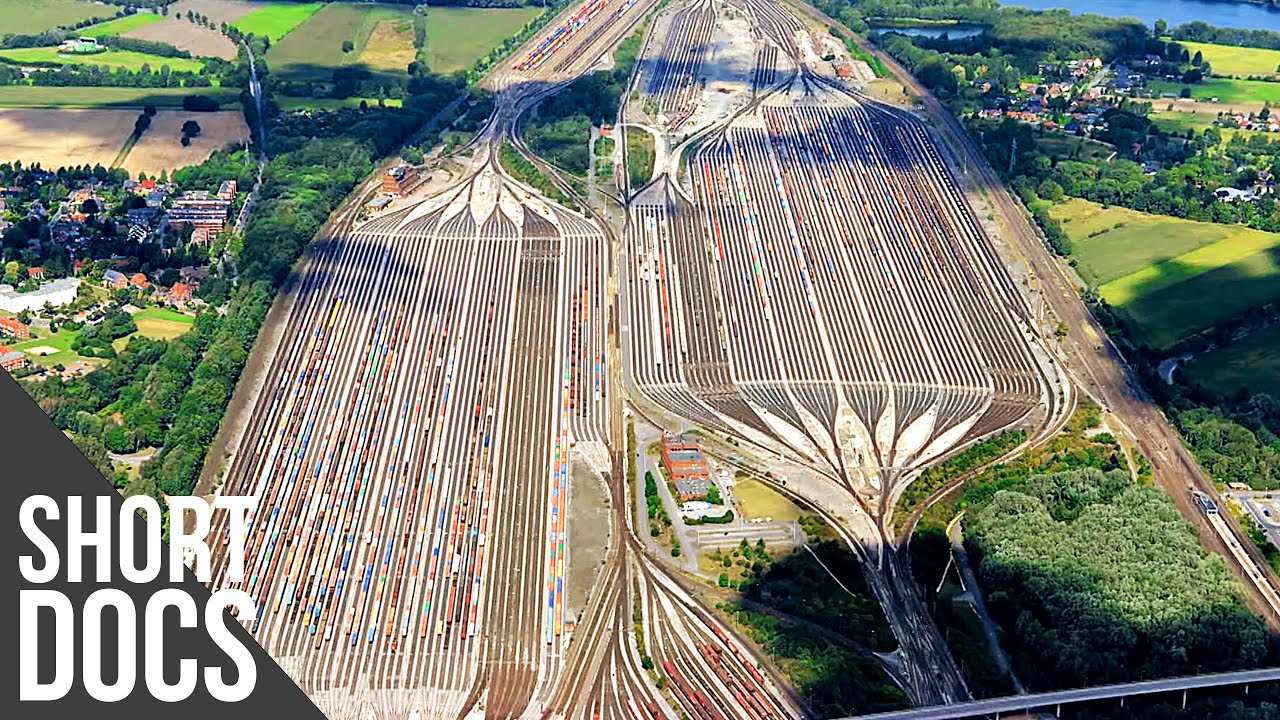
\includegraphics[width=0.7\textwidth]{img/Shuntingyard_real.jpg}
        \caption{Real Shunting Yard (\href{https://www.youtube.com/watch?v=ACNeDxew5Q4&ab_channel=FreeDocBites}{Source})}
      \end{figure}
    \end{column}
  \end{columns}
\end{frame}

\begin{frame}{A simpler case}
  Let's consider a simpler case, we assume the formula we will get only consist of 3 types of things, number, $+$ and $\times$, no subtraction, no division (actually there are by changing the number). We also do not allow parenthesis, whenever there are terms like
  $$a\times b\times c$$
  it is equal to 
  $$(a\times b)\times c$$
  We call this type of rule \textbf{left-associative}.
\end{frame}

\begin{frame}{Idea for implementation I}
  We consider walking through the array from left to right, then we can always see only 3 things by our restriction,
  \begin{itemize}
    \item Numbers: let's first leave this alone since we don't know what to do yet, we continue walking.
    \item $+$: we found an operator, but there might be $\times$ behind and we need to evaluate that first, we continue walking.
    \item $\times$: we found an operator again, and since here $\times$ must have the highest order of evaluation, we can always evaluate it, grab the thing infront and behind to compute it!
  \end{itemize}
\end{frame}

\begin{frame}{Idea for implementation II}
  So you can imagine, after first round of walking, we will evaluate all the $\times$, but the problem is how to keep track of the things infront? What if we encounter things like 
  $$a\times b\times c\times d\times ...$$
  We need something to store the things we walked pass and also be able to \textbf{keep track of} what is the \textbf{last thing added} to the storage and since we are doing this repeatly thus we also want this to be \textbf{efficient} as well.\\
  \begin{center}
    \textbf{Stack is what we need!!!}
  \end{center}
\end{frame}

\begin{frame}{Idea for implementation III}
  So what we will be doing is maintain a stack that stores the the things passed by, then whenever we encounter a $\times$, we pop the last elements stored and multiply it with the next elements in the formula. For example the equation 
  $$1\times 2\times 3$$
  The stack we maintained will be something like
  \begin{figure}[h!]
    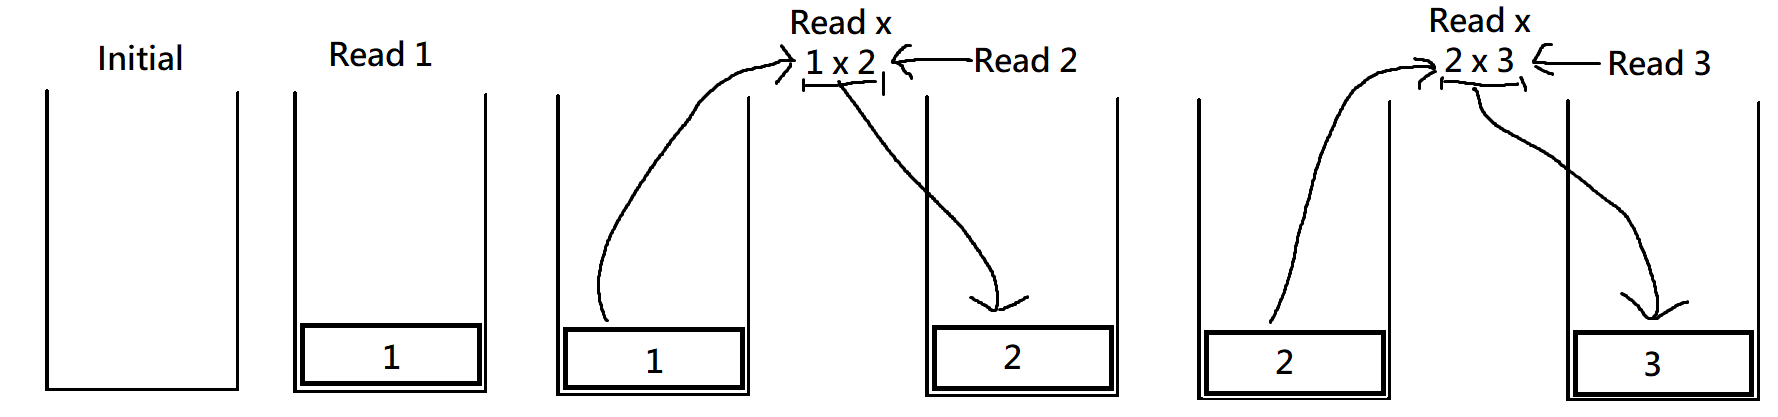
\includegraphics[width=0.7\textwidth]{img/ParserEg.png}
    \caption{Stack state explained (self-drawn)}
  \end{figure}
\end{frame}

\begin{frame}{Idea for implementation IV}
  Now we are left with the last pieces, after the above process, we will obtain a stack that contains of only two types of things:
  \begin{enumerate}
    \item Numbers
    \item Operator $+$
  \end{enumerate}
  Hence we simply pop all of them out and add them up.
\end{frame}

\begin{frame}[fragile]
\begin{lstlisting}[language=python]
def EquationParser(formula):
  tokens=formula.split()
  walked=stack()
  flag=False
  for token in tokens:
    if flag==True:
      left=int(walked.pop())
      right=int(token)
      walked.push(str(left*right))
      flag=False
    elif token!='*':
      walked.push(token)
    else:
      flag=True
  res=0
  while not walked.empty():
    temp=walked.pop()
    if temp!='+':
      res=res+int(temp)
  return res
\end{lstlisting}
\end{frame}

\begin{frame}{Your turn now!}
  Let's have some practices. This time we will have something different, we will borrow the problem from \textbf{HKOI}, the Hong Kong Olympiad of Informatics, for the practice. Please visit the following link
  \begin{center}
    https://judge.hkoi.org/task/01030
  \end{center}
  and login with your \textbf{school} gmail account, read the problem and you can first try to solve the problem on your own computer/Google Colab, then once you are confidence with your solution try to submit it. \\
  Hint: you can try to use the queue here, it will be helpful.
\end{frame}
\end{document}
